\section{\trAdjointFunctorTheorem{}}
\label{sec:adjoint-functor-theorems}

本节的目标是证明两条\trAdjointFunctorTheorem{}，论证沿 \cite{NRS19} 给出。
这两条定理随即在\trPresentable{}（presentable）∞-\trCategories{}的语境中蕴含%
\trLurie{}的\trAdjointFunctorTheorem{} \cite{Lur09}。

\begin{definition}\label{def:colimit-dense}
∞-\trCategory{} $\C$ 的一个满子范畴 $\C_0 \subseteq \C$ 称为%
\emph{余极限稠密的}（colimit-dense），如果 $\C$ 的每个\trObject{}都可以写成某个
图表 $p\colon K \to \C_0 \subseteq \C$ 的\trColimit{}。
\end{definition}

\begin{theorem}\label{thm:adjoint-functor-theorem-colimits}
设 $\C$ 是一个\trLocallySmall{}∞-\trCategory{}，它是\trCocomplete{}，并且含有一个\trEssentiallySmall{}、
余极限稠密的满子范畴 $\C_0 \subseteq \C$。设 $\D$ 是一个\trLocallySmall{}∞-\trCategory{}，
并设 $F\colon \C \to \D$ 是一个\trFunctor{}。那么，$F$ 容有一个\trRightAdjoint{}，
当且仅当 $F$ 保持诸\trColimit{}。
\end{theorem}

\begin{remark}\label{rem:accessible-categories}
容有一个小的、余极限稠密的满子范畴的\trLocallySmall{}∞-\trCategories{}，其例子便是%
\trAccessible{}（accessible）∞-\trCategories{}。称一个∞-\trCategory{}是\emph{\trAccessible{}}%
（accessible），如果它对某个正则基数 $\kappa$ 而言是 $\kappa$-\trAccessible{}。一个
$\kappa$-\trAccessible{}∞-\trCategory{}是一个\trLocallySmall{}∞-\trCategory{} $\C$，它容许
$\kappa$-\trFiltered{}余极限，并且含有一个\trEssentiallySmall{}子范畴 $\C_0$，使得 $\C_0$ 的每个%
\trObject{}都是 $\kappa$-\trCompact{}，而 $\C$ 的每个\trObject{}都是 $\C_0$ 中
诸\trObject{}的一个 $\kappa$-\trFiltered{}余极限。

回忆：$\kappa$-\trFiltered{}余极限指的是对一个\trFunctor{} $f\colon I \to \C$ 取的%
\trColimit{}，其中∞-\trCategory{} $I$ 是 $\kappa$-\trFiltered{}。而这又意味着：任何
图表 $J \to I$ 都容有一个\trCone{} $J \star \Delta^0 \to I$，只要 $J$ 是一个
$\kappa$-小\trSimplicialSet{}（也就是说，其非退化\trSimplex{}的基数小于
$\kappa$）。
\end{remark}

\begin{remark}\label{rem:presentable}
一个此外还\trCocomplete{}\trAccessible{}∞-\trCategory{}称为\emph{\trPresentable{}}%
（presentable）。于是，上述\cref{thm:adjoint-functor-theorem-colimits}便可以应用
于\trPresentable{}∞-\trCategories{}之间的\trFunctor{}，从而\trPresentable{}\trCategories{}之间任何
保持\trColimit{}的\trFunctor{}都容有一个\trRightAdjoint{}。
\end{remark}

在深入\cref{thm:adjoint-functor-theorem-colimits}的证明之前，让我们先陈述它的一个
重要推论。

\begin{corollary}\label{cor:cocomplete-implies-complete}
设 $\C$ 是一个\trLocallySmall{}∞-\trCategory{}，它是\trCocomplete{}，并且含有一个\trEssentiallySmall{}、
余极限稠密的满子范畴 $\C_0 \subseteq \C$。那么，$\C$ 是\trComplete{}。
\end{corollary}

\begin{proof}
设 $K$ 是一个小\trSimplicialSet{}。考虑\trFunctor{}%
$\mathrm{const}\colon \C \to \mathrm{Fun}(K, \C)$，它保持诸\trColimit{}，见
\cref{cor:const-preserves-K-colimits}。此外，$\mathrm{Fun}(K, \C)$ 仍是\trLocallySmall{}（其理由可参见，例如，
\cite[Example 5.4.1.8]{Lur09}）。事实上，可以把\trFunctor{}范畴中从 $F$ 到 $G$
的诸\trMappingSpace{}写成下述复合的\trLimit{}：
\[
\mathrm{Tw}(K) \longrightarrow K^{\mathrm{op}} \times K
  \xrightarrow{\ (F, G)\ } \C^{\mathrm{op}} \times \C
  \xrightarrow{\ \mathrm{map}_{\C}\ } \mathrm{Spc},
\]
然后由「$\mathrm{Tw}(K)$ 是小的」与「这个\trFunctor{}的每个值都是小的」这两个
事实推出：该\trFunctor{}之上的\trLimit{}也是一个小的空间。于是，由%
\cref{thm:adjoint-functor-theorem-colimits}，常值\trFunctor{}容有一个%
\trRightAdjoint{}，而由\cref{rem:limit-adjoint-dual}\footnote{译注：原书引作「Proposition
5.1.24」，按 5.1.24 实为余极限/左伴随方向，极限情形见注 5.1.25，此处径改。
——译者注}，它把图表 $p\colon K \to \C$ 送到 $p$ 的一个%
\trLimit{}。
\end{proof}

为了证明\cref{thm:adjoint-functor-theorem-colimits}，我们需要一些准备工作。我们将
使用下述获取\trRightAdjoint{}的判据。

\begin{proposition}\label{prop:right-adjoint-terminal-slice}
设 $F\colon \C \to \D$ 是一个\trFunctor{}。那么，$F$ 容有一个\trRightAdjoint{}，
当且仅当对 $\D$ 的一切\trObject{} $d$，∞-\trCategory{} $\C_{/d}$ 容有一个%
\trTerminalObject{}。
\end{proposition}

\begin{proof}
设 $d$ 是 $\D$ 的一个\trObject{}，并考虑 $\C_{/d}$ 的一个\trTerminalObject{}，
它由偶对 $(Gd, f)$ 给出，其中 $f$ 是 $\D$ 中一个\trMorphism{} $FGd \to d$。由于
我们想用\cref{prop:right-adjoint-criterion}来证明 $F$ 容有一个\trRightAdjoint{}，我们必须考虑下图中的
下方复合：
\begin{center}
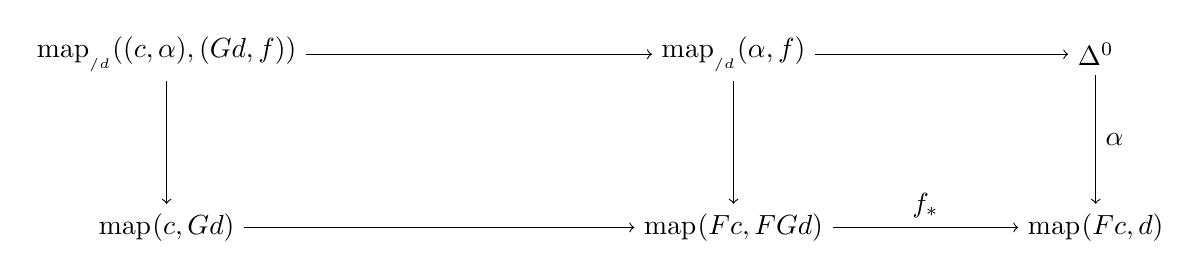
\begin{tikzpicture}
  \node (tl) at (0,0) {$\mathrm{map}_{\C_{/d}}((c, \alpha), (Gd, f))$};
  \node (tm) at (7.2,0) {$\mathrm{map}_{\D_{/d}}(\alpha, f)$};
  \node (tr) at (11.8,0) {$\Delta^0$};
  \node (bl) at (0,-2.2) {$\mathrm{map}_{\C}(c, Gd)$};
  \node (bm) at (7.2,-2.2) {$\mathrm{map}_{\D}(Fc, FGd)$};
  \node (br) at (11.8,-2.2) {$\mathrm{map}_{\D}(Fc, d)$};
  \draw[->] (tl) -- (tm);
  \draw[->] (tm) -- (tr);
  \draw[->] (tl) -- (bl);
  \draw[->] (tm) -- (bm);
  \draw[->] (tr) -- node[right] {$\alpha$} (br);
  \draw[->] (bl) -- (bm);
  \draw[->] (bm) -- node[above] {$f_*$} (br);
\end{tikzpicture}
\end{center}
注意，左边的方块是由下述∞-\trCategories{}的\trPullback{}诱导出的诸%
\trMappingSpace{}的\trPullback{}：
\begin{center}
\begin{tikzpicture}
  \node (cd) at (0,0) {$\C_{/d}$};
  \node (dd) at (2.8,0) {$\D_{/d}$};
  \node (c) at (0,-1.9) {$\C$};
  \node (d) at (2.8,-1.9) {$\D$};
  \draw[->] (cd) -- (dd);
  \draw[->] (cd) -- (c);
  \draw[->] (dd) -- (d);
  \draw[->] (c) -- (d);
\end{tikzpicture}
\end{center}
此外，右边的方块由第 3 章中的\cref{prop:mapping-space-slice}是一个%
\trHomotopy{}\trPullback{}。于是，大方块也是一个\trHomotopy{}\trPullback{}，
而由 $(Gd, f)$ 是 $\C_{/d}$ 的一个\trTerminalObject{}这一假设，上方复合是一个%
\trEquivalence{}。
因此，下方复合在 $\mathrm{map}_{\C}(c, Gd)$ 的所有位于 $\alpha$ 在
$\mathrm{map}_{\D}(Fc, d)$ 中的连通分量之上的连通分量上是\trEquivalence{}。
由于这对一切 $\alpha\colon Fc \to d$ 成立，断言由\cref{prop:right-adjoint-criterion}得出。
\end{proof}

\begin{remark}\label{rem:left-adjoint-initial-slice}
同样地，一个\trFunctor{}容有一个\trLeftAdjoint{}，当且仅当对 $\D$ 的一切%
\trObject{} $d$，\trCategory{} $\C_{d/}$ 容有一个\trInitialObject{}。
\end{remark}

\begin{remark}\label{rem:adjoint-cofinal-coinitial}
由于容有\trTerminalObject{}或\trInitialObject{}的∞-\trCategories{}都是%
\trWeaklyContractible{}，我们可以由第 4 章中的\cref{thm:quillen-theorem-a}
（及其对偶版本）推出：容有一个\trLeftAdjoint{}的\trFunctor{}是\trCofinal{}%
（而容有一个\trRightAdjoint{}的\trFunctor{}是\trCoinitial{}）。
\end{remark}

因此，我们需要找出一些判据，以保证特定的\trCategories{}容有\trTerminalObject{}。
为此，我们将利用\trWeaklyTerminal{}集这一概念。

\begin{definition}\label{def:weakly-terminal}
设 $\C$ 是一个∞-\trCategory{}，并设 $S$ 是一个由\trObject{}组成的（小）集。
称 $S$ 是\emph{\trWeaklyTerminal{}}（weakly terminal），如果对 $\C$ 的每个\trObject{} $x$，
都存在 $S$ 中的一个\trObject{} $s$，使得空间 $\mathrm{map}_{\C}(x, s)$ 非空。
称一个\trObject{} $t$ 是\trWeaklyTerminal{}，如果集合 $\{t\}$ 是一个%
\trWeaklyTerminal{}集。
\end{definition}

\begin{lemma}\label{lem:colimit-dense-weakly-terminal}
设 $\C_0 \subseteq \C$ 是一个\trCocomplete{}\trCategory{}的\trEssentiallySmall{}、余极限
稠密的满子范畴。那么，$\C$ 有一个\trWeaklyTerminal{}\trObject{}。
\end{lemma}

\begin{proof}
考虑\trFunctor{} $\C_0 \to \C$，并选取一个\trJoyalEquivalence{}%
$\C' \simeq \C_0$，其中 $\C'$ 是一个小\trSimplicialSet{}。由于%
\trJoyalEquivalence{}由第 4 章中的\cref{cor:joyal-equiv-cofinal}可知是%
\trCofinal{}，且 $\C$ 是\trCocomplete{}，我们发现\trFunctor{}%
$\C_0 \to \C$ 容许一个\trColimit{} $t$。我们断言：$t$ 是一个\trWeaklyTerminal{}\trObject{}。
为了看出这一点，设 $x$ 是 $\C$ 的另一个\trObject{}。由假设，存在一个\trFunctor{}%
$K \to \C_0$，使得复合 $K \to \C_0 \to \C$ 之上的\trColimit{}由 $x$ 给出。
我们在诸\trColimit{}上得到一个典范映射 $x \to t$。特别地，映射 $x \to t$ 的
空间非空。
\end{proof}

\begin{proposition}\label{prop:weakly-terminal-cofinal}
设 $\C$ 是一个\trLocallySmall{}且\trCocomplete{}∞-\trCategory{}，设 $S$ 是一个\trWeaklyTerminal{}集，
并设 $\C_0$ 是由 $S$ 张成的满子范畴。那么，$\C_0 \to \C$ 是\trCofinal{}。
\end{proposition}

\begin{proof}
由第 4 章中的\cref{thm:quillen-theorem-a}，只需证明：对 $\C$ 的任何\trObject{}%
$x$，切片 $(\C_0)_{x/}$ 是\trWeaklyContractible{}。如果我们能证明：对任何小%
\trSimplicialSet{} $K$，任何\trFunctor{} $K \to (\C_0)_{x/}$ 都穿过那个%
\trContractible{}含入 $K \to K \star \Delta^0$，那么便得出
$(\C_0)_{x/}$ 如所需那样是\trWeaklyContractible{}。为了证明上述陈述，考虑
一个\trFunctor{} $K \to (\C_0)_{x/}$ 以及复合
\[
K \longrightarrow (\C_0)_{x/} \longrightarrow \C_{x/}.
\]
由于 $\C$ 是\trCocomplete{}，由第 4 章中的\cref{prop:fat-slice-cocomplete}，
对 $\C_{x/}$ 亦是如此。因此，我们可以选取上述\trFunctor{}的一个\trColimit{}%
\trCone{}%
\begin{center}
\begin{tikzpicture}
  \node (k) at (0,0) {$K$};
  \node (c0x) at (3.6,0) {$(\C_0)_{x/}$};
  \node (cx) at (7.2,0) {$\C_{x/}$};
  \node (kc) at (0,-2.2) {$K \star \Delta^0$};
  \draw[->] (k) -- (c0x);
  \draw[->] (c0x) -- (cx);
  \draw[->] (k) -- (kc);
  \draw[->] (kc) -- node[below right] {$\mu$} (cx);
\end{tikzpicture}
\end{center}
并考虑 $\mu(\infty)\colon x \to t$。选取 $S$ 中一个使映射 $t \to s$ 存在的%
\trObject{} $s$，并选取这样一个映射。选取 $x \to t$ 与 $t \to s$ 的一个复合，
便给出一个 $2$-\trSimplex{} $\sigma\colon \Delta^2 \to \C$，它伴随于一个映射
$\Delta^1 \to \C_{x/}$。于是我们考虑\trLiftingProblem{}%
\begin{center}
\begin{tikzpicture}
  \node (tl) at (0,0)
    {$K \star \Delta^0 \amalg_{\Delta^0} \Delta^1$};
  \node (tr) at (7.0,0) {$\C_{x/}$};
  \node (bl) at (0,-2.2) {$K \star \Delta^1$};
  \draw[->] (tl) -- node[above] {$(\mu, \sigma)$} (tr);
  \draw[->] (tl) -- (bl);
  \draw[->, dashed] (bl) -- node[above left] {$\mu'$} (tr);
\end{tikzpicture}
\end{center}
它可以求解，因为竖直映射由第 1 章中的\cref{lem:join-box-anodyne}是%
\trInnerAnodyne{}的，而 $\C_{x/}$ 是一个∞-\trCategory{}。沿含入
$K \star \Delta^{\{1\}} \to K \star \Delta^1$ 限制 $\mu'$，便导出一个穿过
$(\C_0)_{x/}$ 的\trFunctor{} $K \star \Delta^0 \to \C_{x/}$：由于
$(\C_0)_{x/} \subseteq \C_{x/}$ 是一个满子范畴，只需看出 $K \star \Delta^0$ 的
全部\trObject{}都进入 $(\C_0)_{x/}$：在 $K$ 上这一点由假设为真，而在\trCone{}点
$\{\infty\}$ 上，按构造得到映射 $x \to s$，它按构造又含于 $(\C_0)_{x/}$ 中。
至此，本命题证毕。
\end{proof}

\begin{corollary}\label{cor:weakly-terminal-terminal-object}
设 $\C$ 是一个\trCocomplete{}\trLocallySmall{}∞-\trCategory{}。假设存在一个\trWeaklyTerminal{}集。
那么，$\C$ 容有一个\trTerminalObject{}。
\end{corollary}

\begin{proof}
设 $S$ 是一个\trWeaklyTerminal{}集，并考虑由 $S$ 张成的满子范畴 $\C_0$。由%
\cref{prop:weakly-terminal-cofinal}，含入 $\C_0 \to \C$ 是\trCofinal{}。
由于 $\C_0$ 是小的，\trFunctor{} $\C_0 \to \C$ 容许一个\trColimit{}。于是，由
第 4 章中的\cref{cor:cofinal-colimit}可以推出：恒同\trFunctor{} $\C \to \C$
也容许一个\trColimit{}。由第 4 章中的\cref{lem:id-colimit-cone-terminal}，
这样一个\trColimit{}是一个\trTerminalObject{}。
\end{proof}

\begin{remark}\label{rem:weakly-initial-initial-object}
通过取相反\trCategories{}，我们发现：若 $\C$ 是一个\trLocallySmall{}且\trComplete{}%
\trCategory{}，并且容有一个\trWeaklyInitial{}集，则它容有一个\trInitialObject{}。
\end{remark}

\begin{proof}[\cref{thm:adjoint-functor-theorem-colimits} 的证明]
「左伴随保持诸\trColimit{}」这一事实已在\cref{prop:left-adjoint-preserves-colimits}中处理过。因此，我们来证明：
若 $F$ 保持诸\trColimit{}，则 $F$ 容有一个\trRightAdjoint{}。
由\cref{prop:right-adjoint-terminal-slice}，只需证明：对 $\D$ 的每个\trObject{}%
$d$，切片 $\C_{/d}$ 有一个\trTerminalObject{}。

为此，我们首先观察到 $\C_{/d}$ 仍是\trLocallySmall{}且\trCocomplete{}。\trCocomplete{}性
由\cref{prop:pullback-colimits}得出：因为按假设\trFunctor{} $\C \to \D$ 保持诸\trColimit{}，而%
\trFunctor{} $\D_{/d} \to \D$ 由第 4 章中的%
\cref{prop:fat-slice-preserve-colimits}保持诸\trColimit{}。为了看出 $\C_{/d}$
仍是\trLocallySmall{}，我们借助 $\C$、$\D$ 与 $\D_{/d}$ 中的诸\trMappingSpace{}来计算：
$\C$ 与 $\D$ 中的那些按假设是\trEssentiallySmall{}，而 $\D_{/d}$ 中的那些由第 3 章中的%
\cref{prop:mapping-space-slice}也是\trEssentiallySmall{}。因此，这个\trPullback{}也是\trEssentiallySmall{}。

于是，由\cref{cor:weakly-terminal-terminal-object}，只需确立\trWeaklyTerminal{}\trObject{}的
存在性，而这我们将借助\cref{lem:colimit-dense-weakly-terminal}来导出。换言之，
我们必须证明：$\C_{/d}$ 含有一个\trEssentiallySmall{}、余极限稠密的满子范畴。我们断言：
$(\C_0)_{/d}$ 就是这样一个子范畴。如上所示，$(\C_0)_{/d}$ 是\trLocallySmall{}，从而只需
证明诸\trObject{}的等价类构成一个小的集合。这一点容易由下述事实得出：
$(\C_0)_{/d}$ 的\trObject{}由形如 $(x, \alpha\colon F(x) \to d)$ 的偶对给出，
其中 $x \in \C_0$。由于 $\C_0$ 是\trEssentiallySmall{}，这样的 $x$ 的等价类构成一个小集。
此外，对每个这样的 $x$，映射空间 $\mathrm{map}_{\D}(F(x), d)$ 也因 $\D$ \trLocallySmall{}%
这一假设而是\trEssentiallySmall{}。因此，剩下要证的是 $(\C_0)_{/d} \to \C_{/d}$ 是一个余极限
稠密的子范畴。为此，设 $(y, \alpha\colon F(y) \to d)$ 是 $\C_{/d}$ 的一个%
\trObject{}，并写 $y = \mathrm{colim}_K p$，其中 $p\colon K \to \C_0 \subseteq \C$
是某个图表。现在我们证明：这个图表可以被提升为一个图表
$p'\colon K \to (\C_0)_{/d}$。为了做到这一点，我们首先注意：映射
$K \to \C_0 \xrightarrow{\ i\ } \C$ 的一个\trColimit{}\trCone{}给出一个映射
$K \to \C_{/y}$。把这个映射与 $F$ 复合，便得到一个映射 $K \to \D_{/F(y)}$，而
映射 $\alpha$ 进而给出一个映射 $\D_{/F(y)} \to \D_{/d}$。于是我们找到一个图表
\begin{center}
\begin{tikzpicture}
  \node (k) at (0,0) {$K$};
  \node (dd) at (3.4,0) {$\D_{/d}$};
  \node (c0) at (0,-2.0) {$\C_0$};
  \node (d) at (3.4,-2.0) {$\D$};
  \draw[->] (k) -- node[above] {$g$} (dd);
  \draw[->] (k) -- node[right] {$p$} (c0);
  \draw[->] (dd) -- (d);
  \draw[->] (c0) -- node[above] {$F\iota$} (d);
\end{tikzpicture}
\end{center}
它按构造交换。于是我们得到一个诱导映射 $p'\colon K \to (\C_0)_{/d}$，它与
$(\C_0)_{/d} \to \C_{/d}$ 的复合正是图表 $p$。为了完成本定理的证明，现在只需
注意：$p'$ 的\trColimit{}可以由第 4 章中的\cref{prop:fat-slice-preserve-colimits}
计算得 $(y, \alpha)$。
\end{proof}

我们以「\trPresentable{}∞-\trCategories{}所能享有的另一条\trAdjointFunctorTheorem{}」来为
本书作结。为此，回忆：称一个∞-\trCategory{}是\trAccessible{}，如果它对某个基数 $\kappa$
是 $\kappa$-\trAccessible{}；称一个\trFunctor{}是\trAccessible{}，如果它对某个基数 $\kappa$ 是
$\kappa$-\trAccessible{}，也就是说，如果它对某个足够大的基数 $\kappa$ 保持
$\kappa$-\trFiltered{}余极限。

\begin{theorem}\label{thm:adjoint-functor-theorem-limits}
设 $\C$ 是一个\trLocallySmall{}、\trAccessible{}且\trComplete{}∞-\trCategory{}，并设 $\D$ 是一个%
\trLocallySmall{}且\trComplete{}∞-\trCategory{}，其中每个\trObject{}对某个 $\kappa$
而言都是 $\kappa$-\trCompact{}。那么，若\trFunctor{} $F\colon \C \to \D$ 保持
诸\trLimit{}并且是\trAccessible{}，则 $F$ 容有一个\trLeftAdjoint{}。
\end{theorem}

\begin{proof}
我们想证明：对 $\D$ 的一切\trObject{} $d$，切片 $\C_{d/}$ 有一个%
\trInitialObject{}。由\cref{cor:weakly-terminal-terminal-object}的对偶版本，
只需证明 $\C_{d/}$ 容有一个\trWeaklyInitial{}集。（注意，$\C_{d/}$ 是\trLocallySmall{}且\trComplete{}，
因为 $\C$ 与 $\D$ 按假设是\trComplete{}，而且 $F\colon \C \to \D$ 与
$\D_{d/} \to \D$ 二者都保持诸\trLimit{}。）我们固定一个正则基数 $\kappa$，使得
下述条件成立：
\begin{enumerate}[label=(\arabic*)]
  \item $\C$ 是 $\kappa$-\trAccessible{}，
  \item $F$ 是 $\kappa$-\trAccessible{}，
  \item $d$ 是 $\kappa$-\trCompact{}。
\end{enumerate}
对每一项而言，这样的 $\kappa$ 都由诸假设保证存在，而通过换成适当大的基数，
我们还能找到一个同时满足所有这三个条件的基数，见下文\cref{rem:cardinal-facts}。

接下来，我们考虑 $\C_{d/}$ 的诸\trObject{}组成之集 $S$，它由全部形如
$(x, \alpha\colon d \to Fx)$ 的偶对构成，其中 $x$ 是 $\C$ 的一个%
$\kappa$-\trCompact{}\trObject{}。由于 $\C$ 的诸 $\kappa$-\trCompact{}%
\trObject{}组成的子范畴 $\C^{\kappa}$ 是\trEssentiallySmall{}，$S$ 实际上是一个小集。我们
断言：集合 $S$ 是\trWeaklyInitial{}。为了看出这一点，我们考虑 $\C_{d/}$ 的任意一个%
\trObject{} $(z, \beta\colon d \to Fz)$。由于 $\C$ 是 $\kappa$-\trAccessible{}，我们
可以把 $z$ 写成某个图表 $p\colon K \to \C^{\kappa} \subseteq \C$ 的
$\kappa$-\trFiltered{}余极限。由于 $F$ 是 $\kappa$-\trAccessible{}，我们发现
$Fz = \mathrm{colim}_K Fp$。于是，由于 $d$ 是 $\kappa$-\trCompact{}，我们
发现映射
\[
\mathrm{colim}_K\, \mathrm{map}_{\D}(d, Fp(-))
  \longrightarrow \mathrm{map}_{\D}(d, Fz)
\]
是一个\trEquivalence{}。因此，$\beta$ 必定来自某个
$\mathrm{map}_{\D}(d, Fp(k))$，其中 $k$ 是 $K$ 的一个\trObject{}。由于 $p$ 的像
落在诸 $\kappa$-\trCompact{}\trObject{}之中，这个映射出现于集合 $S$ 之中。这就
表明 $S$ 如所断言的那样是\trWeaklyInitial{}，从而证明了本定理。
\end{proof}

\begin{remark}\label{rem:right-adjoint-accessible}
可以证明：在\cref{thm:adjoint-functor-theorem-limits}的假设之下，一个%
\trRightAdjoint{}是\trAccessible{}，可参见，例如，\cite[Theorem 4.1.4 (1)]{NRS19}。
于是，这个陈述可以提升为一条「当且仅当」陈述，因为我们在\cref{prop:left-adjoint-preserves-colimits}中论证过：
\trRightAdjoint{}保持诸\trLimit{}。
\end{remark}

\begin{remark}\label{rem:aft-limits-presentable}
由\cref{cor:cocomplete-implies-complete}，\trPresentable{}∞-\trCategories{}都是%
\trComplete{}，所以我们可以把\cref{thm:adjoint-functor-theorem-limits}应用
于一个\trPresentable{}∞-\trCategory{} $\C$。此外，一个\trAccessible{}（特别是\trPresentable{}）%
∞-\trCategory{} $\D$ 也具有如下性质：任何\trObject{}对某个 $\kappa$ 都是
$\kappa$-\trCompact{}。总而言之，\cref{thm:adjoint-functor-theorem-limits}可以
应用于\trPresentable{}∞-\trCategories{}之间一个\trAccessible{}且保持诸\trLimit{}的\trFunctor{}。
结论是：这样的\trFunctor{}容有一个\trLeftAdjoint{}。
\end{remark}

\begin{remark}\label{rem:cardinal-facts}
在\cref{thm:adjoint-functor-theorem-limits}的证明中，我们随意使用了关于%
\trAccessible{}%
∞-\trCategories{}与\trCompact{}\trObject{}的若干事实，这里随后把它们总结一下。
为此，设 $\kappa' > \kappa$ 是正则基数。那么我们有下述性质：
\begin{enumerate}[label=(\arabic*)]
  \item 任何 $\kappa$-\trCompact{}\trObject{}也是 $\kappa'$-\trCompact{}：
        这仅仅是因为任何 $\kappa'$-\trFiltered{}图表也是 $\kappa$-\trFiltered{}。
  \item 一个 $\kappa$-\trAccessible{}\trFunctor{}也是 $\kappa'$-\trAccessible{}：这同样由「每个
        $\kappa'$-\trFiltered{}图表都是 $\kappa$-\trFiltered{}」这一事实得出。
  \item 一个 $\kappa$-\trAccessible{}∞-\trCategory{}一般不必是 $\kappa'$-\trAccessible{}，
        见 \cite[Remark 5.4.2.12]{Lur09}。然而，总可以找到许多
        $\kappa'' > \kappa$，使得一个 $\kappa$-\trAccessible{}∞-\trCategory{}也是
        $\kappa''$-\trAccessible{}，见 \cite[Proposition 5.4.2.11]{Lur09}。
\end{enumerate}
\end{remark}

\begin{remark}\label{rem:no-completeness-assumption}
\cref{thm:adjoint-functor-theorem-limits}在去掉「$\D$ 是\trComplete{}」这一
假设后仍然成立，见 \cite[proof of Theorem 4.1.1 (2)]{NRS19}。
\end{remark}

\begin{corollary}\label{cor:accessible-complete-presentable}
设 $\C$ 是一个\trLocallySmall{}、\trAccessible{}且\trComplete{}∞-\trCategory{}。那么，$\C$ 是%
\trPresentable{}。
\end{corollary}

\begin{proof}
我们需要证明 $\C$ 是\trCocomplete{}。为此，考虑一个小\trSimplicialSet{} $K$
与常值\trFunctor{} $\C \to \mathrm{Fun}(K, \C)$。如前所述，$\mathrm{Fun}(K, \C)$
结果是\trLocallySmall{}，且每个\trObject{}对某个 $\kappa$ 而言都是 $\kappa$-\trCompact{}，
见 \cite[Proposition 5.3.4.13]{Lur09}。于是我们可以应用%
\cref{thm:adjoint-functor-theorem-limits}并断定：常值\trFunctor{}容有一个%
\trLeftAdjoint{}。因此，由\cref{prop:colimit-adjoint}，$\C$ 容许 $K$-指标的余极限。
\end{proof}
